%% ==================== 方法（扩展版，中文版） ====================
\section{方法}
\label{sec:method}

\subsection{符号与约定}
\textbf{符号约定.} 上标表示感官模态（$^{\text{vis}}$：视觉，$^{\text{imu}}$：惯性，$^f$：融合）或细胞类型（$^g$：网格细胞，$^h$：头方向细胞）。下标 $t$ 表示时间。粗体大写字母表示矩阵或高维数组；粗体小写字母表示向量；花体表示集合。

\subsection{框架架构与全局状态空间表述}
\label{sec:framework_arch}

\begin{figure*}[!htbp]
    \centering
    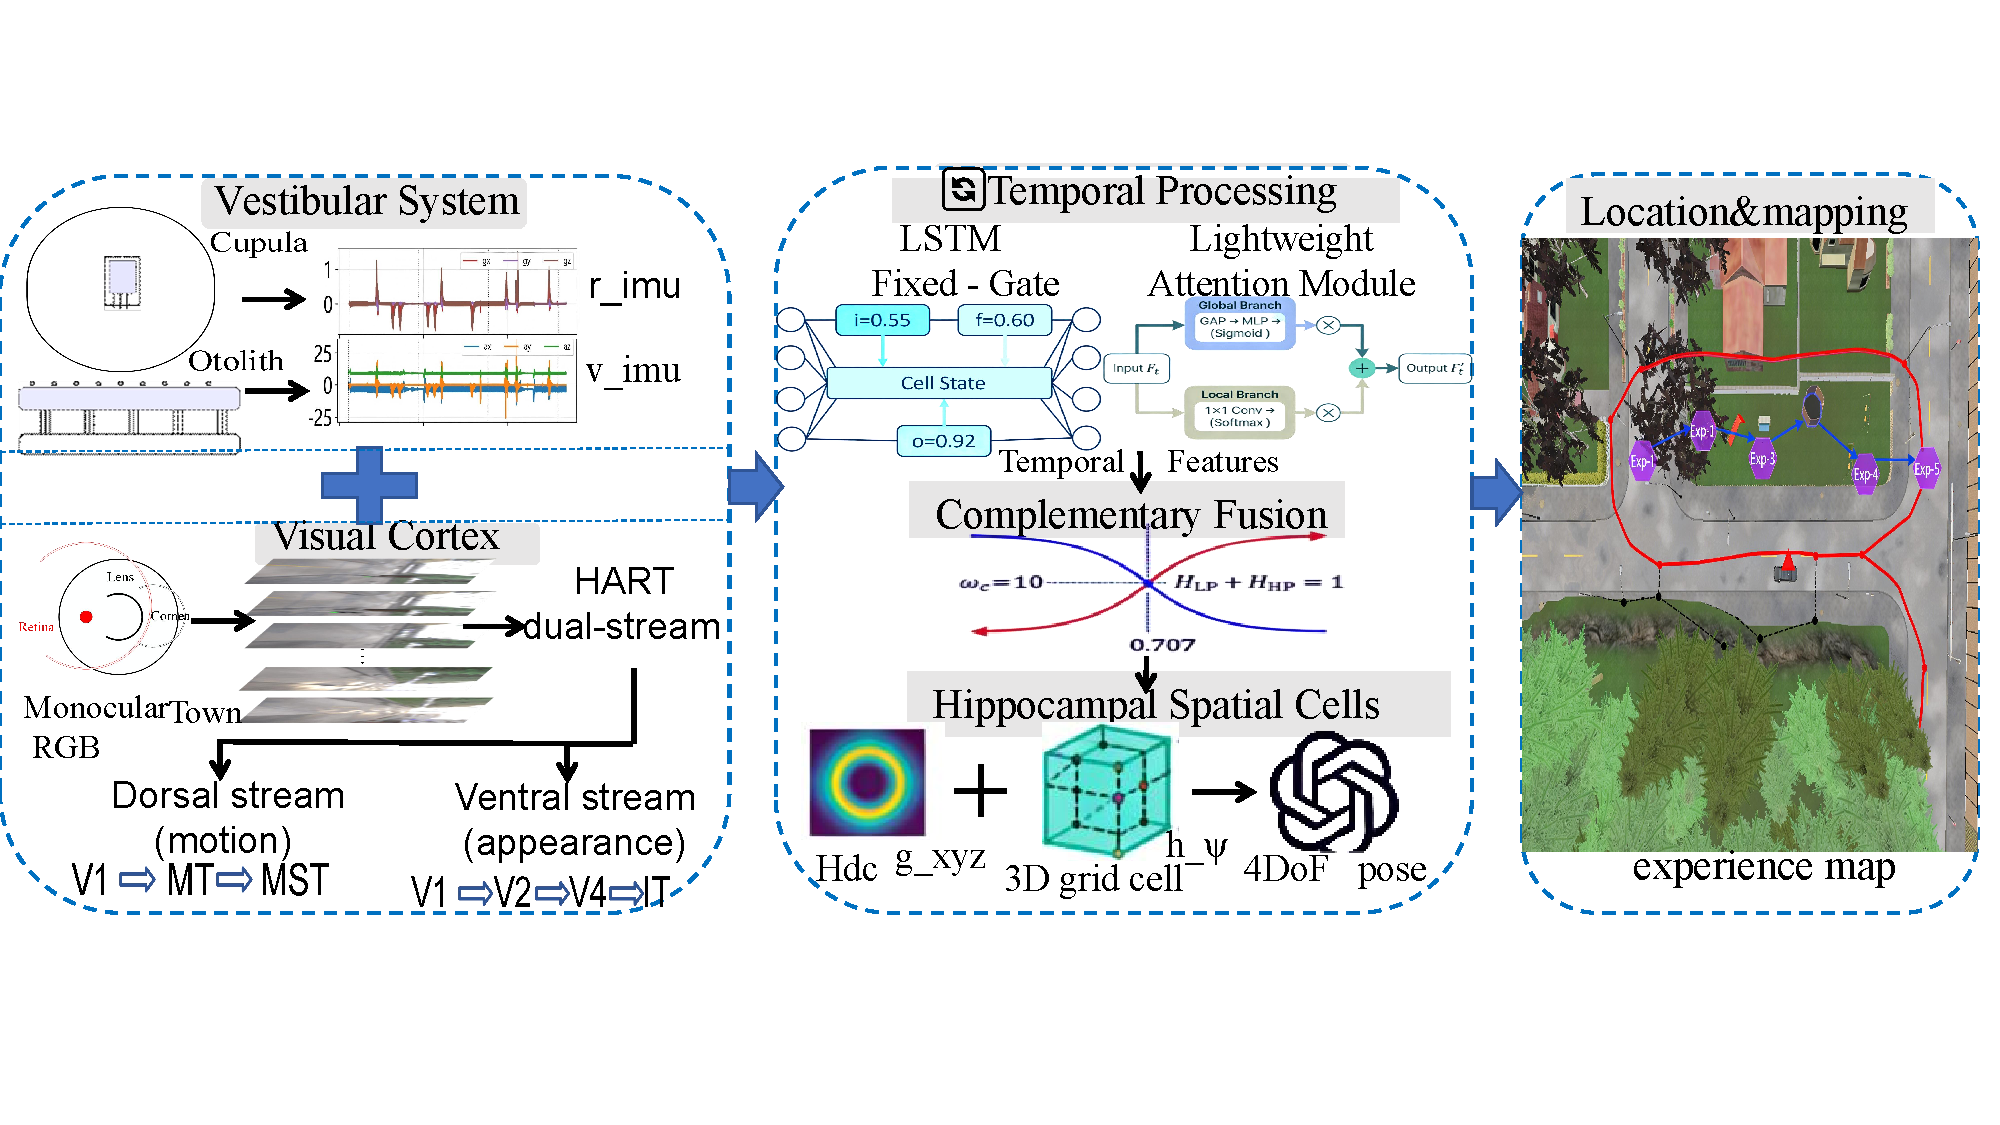
\includegraphics[width=0.95\textwidth]{fig/2_framework.pdf}
    \caption{所提出的多模态视觉-惯性框架的自包含端到端数据流。原始输入为单目RGB图像与IMU测量值。视觉模块将信号分为场景识别与运动估计两支路；前庭模块输出高频惯性运动。两种模态通过频域互补滤波融合。融合后的运动学驱动空间网络更新统一定义于式~\eqref{eq:global_state} 的4自由度全局状态 $\mathbf{X}_t$。经验图模块执行闭环松弛以消除长期轨迹漂移。所有子模块共享本小节提出的标准化状态空间变量。}
    \label{fig:system_overview}
\end{figure*}
本工作为机器人定位设计了一个多模态视觉-惯性信号处理系统，它由三个紧耦合的功能子系统组成：分层多尺度视觉特征算子、前庭-惯性传感器状态估计器、度量空间状态编码网络。与传统的基于EKF的松耦合框架不同，所提出的系统采用频域互补融合来解耦低频视觉观测噪声与高频惯性瞬态噪声，并通过连续吸引子空间网络更新全局度量状态以抑制长期轨迹漂移。

\subsubsection{全局离散状态空间模型}
为后续所有子模块推导提供统一的数学基础，我们首先定义 $t$ 时刻系统的离散状态空间表示。

1) 多模态原始输入向量
\begin{equation}
    \mathbf{U}_t = \left[ I_t,\, \mathbf{a}_t^\top,\, \boldsymbol{\omega}_t^\top \right]
    \label{eq:input_vec}
\end{equation}
其中 $I_t$ 表示采集的单目RGB图像；$\mathbf{a}_t$ 与 $\boldsymbol{\omega}_t$ 分别为加速度计线加速度与陀螺仪角速度测量值。

2) 核心4自由度全局位姿状态向量
\begin{equation}
    \mathbf{X}_t = \left[ x_t,\, y_t,\, z_t,\, \psi_t \right]^\top \in \mathbb{R}^3 \times \mathrm{SO}(2)
    \label{eq:global_state}
\end{equation}
在该表述中，$(x_t, y_t, z_t) \in \mathbb{R}^3$ 表示全局3D平移坐标（单位：米），$\psi_t \in [-\pi,\pi)$ 表示水平偏航角（单位：弧度）。

3) 统一状态演化映射函数
\begin{equation}
    \mathbf{X}_{t+1} = \mathcal{F}\big(\mathbf{X}_t,\, \mathbf{U}_t\big)
    \label{eq:state_evolution}
\end{equation}
映射 $\mathcal{F}(\cdot)$ 封装了完整的前向流水线，包括多尺度视觉特征提取、惯性运动计算、频域多模态融合与空间网络路径积分。$\mathcal{F}(\cdot)$ 的详细数学分解将在3.3节（视觉-前庭处理）与3.4节（空间编码网络）中给出。

如图~\ref{fig:system_overview} 所示，端到端数据流水线由五个顺序耦合的模块组成：
1. 分层双流视觉前端：构建并行的腹侧/背侧支路，分别独立生成场景描述子并计算逐像素自运动，消除识别与跟踪任务间的相互干扰。
2. 前庭IMU处理模块：从原始惯性数据中推导高频瞬态运动信号，无需迭代式在线偏置标定。
3. 互补融合单元：采用一阶IIR滤波器分离低频视觉漂移与高频惯性噪声，输出平滑的平移与旋转运动学量。
4. 度量空间编码网络：使用融合运动线索更新分布式空间细胞状态，并通过视觉模板锚定约束抑制积分漂移。
5. 拓扑经验图：记录历史视觉描述子与空间细胞快照，在检测到闭环时执行一次全局图松弛，以保证全局一致的度量位姿。

\subsection{感官处理与融合}

感官处理模块从视觉与惯性模态中提取自运动线索，然后通过互补滤波进行融合。

\textbf{视觉前端.} 视觉前端实现了受灵长类视觉皮层分层架构启发的生物学合理处理流水线，将原始RGB图像转化为适合地点识别与运动估计的紧凑场景描述子。

\textbf{分层特征提取.} 给定RGB图像 $I_t\in\mathbb{R}^{H\times W\times 3}$，我们定义一组模仿从视网膜到颞下皮层各处理阶段的算子。

\textbf{阶段1：视网膜与LGN处理.} 初始预处理模拟视网膜与外侧膝状体（LGN）的早期视觉处理：
\begin{align}
     & \text{亮度通道：}\quad Y_t = \mathcal{G}(I_t) = 0.299R+0.587G+0.114B              \\
     & \text{局部对比度增强：}\quad U_t = \mathcal{C}_\lambda(Y_t),\quad \lambda=0.02 \\
     & \text{感受野模拟：}\quad V_t = U_t * \mathcal{K}_\sigma,\quad \sigma=0.5
\end{align}
其中 $\mathcal{G}$ 为灰度转换算子，$\mathcal{C}_\lambda$ 为限幅对比度自适应直方图均衡（CLAHE），限幅为 $\lambda$；$\mathcal{K}_\sigma$ 为标准差 $\sigma$ 的高斯核。CLAHE在自适应增强局部对比度的同时防止噪声被过度放大，模仿视网膜神经节细胞的中心-周围拮抗组织结构。

\textbf{阶段2：初级视觉皮层（V1-V4）处理.} 中层处理对表征进行归一化与标准化：
\begin{align}
     & \text{动态范围归一化：}\quad \tilde V_t = \frac{V_t-\min(V_t)}{\max(V_t)-\min(V_t)}     \\
     & \text{空间标准化：}\quad Z_t = \mathcal{D}(\tilde V_t)\in\mathbb{R}^{64\times64}        \\
     & \text{局部均值减去：}\quad Z_t(i,j)\leftarrow Z_t(i,j)-\frac{1}{64}\sum_{k=1}^{64}Z_t(i,k)
\end{align}
其中 $\mathcal{D}$ 为下采样算子（双线性插值）。按行减去均值可去除全局强度变化同时保留局部空间结构，类似于V1与V2中的除性归一化。

\textbf{阶段3：颞下（IT）表征.} 最终表征为紧凑的向量化描述子：
\begin{equation}
    \boldsymbol{\phi}_t=\mathrm{vec}(Z_t)\in\mathbb{R}^{4096}
\end{equation}
其中 $\mathrm{vec}(\cdot)$ 表示将二维特征图映射为一维描述子的向量化算子，$\boldsymbol{\phi}_t$ 为时间戳 $t$ 处的整体场景特征向量。
该 $64 \times 64 = 4096$ 维特征向量作为整体场景描述子，类似于IT皮层中视图选择、位置不变的表征。

\textbf{视觉模板匹配与地点识别.} 地点识别通过基于余弦相似度的模板匹配实现，其鲁棒性优于绝对差之和（SAD）等基于强度的度量：
\begin{equation}
    d_{\cos}(\boldsymbol{\phi}_t,\boldsymbol{\phi}_i)=1-\frac{\boldsymbol{\phi}_t^\top\boldsymbol{\phi}_i}{\lVert\boldsymbol{\phi}_t\rVert\,\lVert\boldsymbol{\phi}_i\rVert}
\end{equation}
当当前场景与所有现有模板均足够不同时，创建新的视觉模板（VT）：
\begin{equation}
    \text{若 }\min_{i \in \mathcal{VT}} d_{\cos}(\boldsymbol{\phi}_t, \boldsymbol{\phi}_i)>\tau_{vt}\text{ 则创建新VT},\quad \tau_{vt}=0.08
\end{equation}
阈值 $\tau_{vt}=0.08$ 显著低于传统取值（OpenRatSLAM中的0.15），使相似场景间的判别更精细。实验验证表明，这可使模板数量增加最多39倍（城市环境中从5个增至195个），提供更丰富的地点表征。

\textbf{双流架构与受生物启发的时序建模.} 在上述分层特征提取的基础上，我们的视觉处理融入了两项关键的受生物启发创新：(1) 模仿腹侧/背侧通路的双流架构；(2) 无需训练数据、用于时序一致性的固定门LSTM。

\textbf{双流视觉处理.}
遵循生物视觉双流理论~\cite{Goodale1992, Mishkin1983}，我们从V1输出显式建模两条并行处理通路：

\textbf{背侧通路}（“where”通路，V1$\rightarrow$MT$\rightarrow$MST）：通过基于梯度的特征处理空间位置与运动信息：
\begin{equation}
    \mathbf{F}^{\text{dorsal}}_t = 0.6 \cdot \|\nabla Z_t\| + 0.4 \cdot Z_t
\end{equation}
其中 $\|\nabla Z_t\|$ 为通过Sobel算子计算的梯度幅值，捕获边缘方向与运动方向，类似于MT/MST神经元。

\textbf{腹侧通路}（“what”通路，V1$\rightarrow$V4$\rightarrow$IT）：通过纹理与对比度处理物体身份与场景特征：
\begin{equation}
    \mathbf{F}^{\text{ventral}}_t = 0.4 \cdot Z_t + 0.3 \cdot \sigma_{\text{local}}(Z_t) + 0.3 \cdot \mathcal{C}_\lambda(Z_t)
\end{equation}
其中 $\sigma_{\text{local}}$ 计算局部标准差（纹理特征），$\mathcal{C}_\lambda$ 提供对比度增强，模仿V4对复杂特征的选择性与IT的不变物体表征。

随后，两条支路通过一种轻量全局-局部特征调制机制（详见第~\ref{sec:related_learning} 节）进行集成，该机制使用全局统计量而非完整 Query-Key-Value 运算来近似自注意力效果，保持 $\mathcal{O}(N)$ 复杂度以满足实时性能。

\textbf{用于零样本时序建模的固定门LSTM.}
与需要在领域特定数据集上大量训练的传统数据驱动LSTM不同，我们的时序模块采用人工调定的固定门值，灵感来自生物学前庭-视觉整合原理~\cite{Angelaki2004, Cullen2012}：
\begin{align}
    \text{输入门: }  & i_t = 0.55 \quad \text{（控制新信息摄入）} \\
    \text{遗忘门: } & f_t = 0.60 \quad \text{（保留60\%历史上下文）} \\
    \text{输出门: } & o_t = 0.92 \quad \text{（强调当前感知）}
\end{align}
其中 $i_t$、$f_t$、$o_t$ 分别为受生物启发的LSTM模块的固定输入门、遗忘门、输出门。

该设计为SLAM应用提供了三个关键优势：

\textbf{(1) 零样本部署能力：} 无需训练数据，可立即部署到新环境。这对SLAM至关重要，因为每个环境都有独特的视觉特性，且收集有代表性的训练数据并不可行。我们在六个多样化场景（城市、高速公路、室内）上不做任何环境特定调优的验证，展示了其鲁棒的泛化能力。

\textbf{(2) 生物学可解释性：} 门值反映了神经科学中经实证验证的原则。遗忘门（$f_t=0.6$）实现了与海马重放动力学一致的短期空间记忆保持，其中近期经验被优先保留用于路径积分。高输出门（$o_t=0.92$）优先处理当前感觉输入，模仿前庭系统对即时自运动线索在平衡与导航中的强调。中等输入门（$i_t=0.55$）在新奇检测与稳定性之间取得平衡。

\textbf{(3) 计算效率：} 消除了训练开销（无反向传播、无梯度计算），同时保持实时性能（约31 FPS）。固定门可直接在硬件（如FPGA、神经形态芯片）上实现，无需权重存储或更新逻辑，使其能在资源受限平台上部署。

LSTM按序处理融合后的背侧-腹侧特征，跨时间步维持隐藏状态 $\mathbf{H}_t$ 与细胞状态 $\mathbf{C}_t$：
\begin{align}
    \mathbf{C}_t & = f_t \odot \mathbf{C}_{t-1} + i_t \odot \tanh(\mathbf{F}^{\text{fused}}_t) \\
    \mathbf{H}_t & = o_t \odot \tanh(\mathbf{C}_t)
\end{align}
其中 $\odot$ 表示逐元素Hadamard积，$\mathbf{C}_t$ 为LSTM细胞状态，$\mathbf{H}_t$ 为时序隐藏状态，$\mathbf{F}^{\text{fused}}_t$ 集成了腹侧与背侧视觉特征。

\textbf{与基于学习方法对比.} 第~\ref{sec:experiments} 节表明，我们的固定门LSTM取得了与NeuroSLAM学习得到的LSTM相当或更优的性能（RMSE改善55\%），同时提供零样本部署能力。这验证了：当底层任务结构与生物机制一致时，有原则的受生物启发设计可以匹配甚至超越数据驱动学习——在本例中即是空间导航，生物系统已在数百万年的进化中形成高度优化的解决方案。

\textbf{视觉运动提取.} 除场景识别外，视觉前端还从光流中提取自运动线索，模仿MST（内侧上颞区）的背侧通路处理。

\textbf{特征跟踪与光流计算.} 设 $\mathbf{K}\in\mathbb{R}^{3\times 3}$ 为相机内参矩阵。我们在相邻帧间跟踪 $N$ 个特征点 $\mathbf{p}_i^t\in\mathbb{R}^2$（如使用KLT跟踪）。将跟踪点归一化到相机坐标：
\begin{equation}
    \tilde{\mathbf{q}}_i^t = \mathbf{K}^{-1}\begin{bmatrix}\mathbf{p}_i^t\\ 1\end{bmatrix},\qquad \mathbf{q}_i^t = \pi(\tilde{\mathbf{q}}_i^t)=\frac{1}{\tilde{q}_{i,3}^t}\begin{bmatrix}\tilde{q}_{i,1}^t\\ \tilde{q}_{i,2}^t\end{bmatrix}
\end{equation}
其中 $\pi$ 为透视投影。计算像平面光流：
\begin{equation}
    \mathbf{f}_i=\mathbf{q}_i^t-\mathbf{q}_i^{t-1},\quad \mathbf{q}_i\equiv\mathbf{q}_i^{t-1}
\end{equation}

\textbf{旋转估计.} 对帧间小旋转，归一化点 $\mathbf{q}=(x,y)$ 处偏航引起的流为 $\Delta t\,r\,[-y,\,x]^\top$。我们用加权最小二乘估计视觉偏航角速度：
\begin{equation}
    r^\mathrm{vis}_t=\frac{\sum_{i=1}^N w_i(x_i f_{i,y}-y_i f_{i,x})}{\Delta t\,\sum_{i=1}^N w_i(x_i^2+y_i^2)}
\end{equation}
其中 $w_i$ 为Huber鲁棒权重以抑制离群特征点，$N$ 为跟踪特征总数，$r_t^\mathrm{vis}$ 为视觉估计的偏航角速度。

\textbf{平移估计.} 去除旋转分量以获得平移主导的残余光流：
\begin{equation}
    \mathbf{f}_i^{\perp}=\mathbf{f}_i-\Delta t\,r^\mathrm{vis}_t\begin{bmatrix}-y_i\\ x_i\end{bmatrix}
\end{equation}
假设存在主导地面平面，内点的逆深度为 $\lambda_i\approx 1/Z_g$，则平移流模型为：
\begin{equation}
    \mathbf{f}_i^{\perp}\approx \Delta t\,\lambda_i\,\underbrace{\begin{bmatrix}-1 & 0 & x_i\\ 0 & -1 & y_i\end{bmatrix}}_{\mathbf{A}_i}\,\mathbf{v}^\mathrm{vis}_t,\quad \mathbf{v}^\mathrm{vis}_t=(v_x^\mathrm{vis}, v_y^\mathrm{vis}, v_z^\mathrm{vis})^\top
\end{equation}
带鲁棒权重 $w_i$ 的加权最小二乘解为：
\begin{equation}
    \bar{\mathbf{v}}^\mathrm{vis}_t=\Big(\sum_i w_i\,(\Delta t\,\lambda_i)^2\,\mathbf{A}_i^\top\mathbf{A}_i\Big)^{-1}\,\sum_i w_i\,(\Delta t\,\lambda_i)\,\mathbf{A}_i^\top\mathbf{f}_i^{\perp}
\end{equation}
最终视觉里程计速度引入尺度因子 $\kappa_t$：
\begin{equation}
    \mathbf{v}^\mathrm{vis}_t=\kappa_t\,\bar{\mathbf{v}}^\mathrm{vis}_t
    \label{eq:vis_scale}
\end{equation}
其中 $\lambda_i$ 为特征点 $i$ 的逆深度，矩阵 $\mathbf{A}_i$ 为几何投影矩阵，$\bar{\mathbf{v}}_t^\mathrm{vis}$ 为从光流解出的原始平移速度，$\kappa_t$ 为视觉里程计的在线尺度校正因子。

\textbf{前庭前端.} 前庭前端处理惯性测量值以提取自运动线索，类比哺乳动物的前庭系统。前庭器官由半规管（角速度）与耳石器（线加速度）组成。

\textbf{角速度提取.} 由陀螺仪测量值 $\mathbf{g}_t\in\mathbb{R}^3$（IMU坐标系），我们直接使用 $z$ 轴陀螺而不做在线偏置去除，并按实现转换为度/秒。在平面约束下的4自由度定位-建图中，偏航（方位角）角速度近似为
\begin{equation}
    r_t \approx \mathbf{e}_z^\top\,\boldsymbol{\omega}_t^g,\quad \mathbf{e}_z=(0,0,1)^\top.
\end{equation}
其中 $\boldsymbol{\omega}_t^g$ 为IMU测得的原始陀螺角速度向量，$\mathbf{e}_z$ 为单位竖直基向量。
这对应水平半规管线索，足以满足我们与视觉的互补融合需求。

\textbf{线加速度使用（简化）.} 我们采用与代码库一致的轻量近似：使用加速度计幅值与 $z$ 轴读数，减去常数重力 $g\!=\!9.81$，在帧间隔 $\Delta t$ 上推导指示性的平移与垂向速度分量：
\begin{align}
    v^\mathrm{imu}_{trans}(t) & \approx \max\big(0, (\lVert\mathbf{a}_t\rVert - g)\,\Delta t\,k_t\big), \\
    v^\mathrm{imu}_{z}(t)     & \approx (a_{t,z} - g)\,\Delta t\,k_z,
\end{align}
其中 $g=9.81\,\mathrm{m/s^2}$ 为重力加速度，$k_t, k_z$ 为与实现常数匹配的常值缩放增益，$\Delta t$ 为帧采样间隔。这避免了显式偏置/重力向量估计，同时提供随后通过互补融合与视觉里程计结合的高频运动线索。

\textbf{偏置估计.} 基线实现不进行在线偏置或重力向量估计。更先进的偏置/重力补偿可作为未来工作集成，但对于此处报告的互补融合结果并非必需。

\textbf{互补IMU-视觉融合.} 视觉与惯性模态提供互补信息：视觉里程计提供精确的低频位置估计但长期会漂移，而IMU积分提供可靠的高频运动线索但会累积偏置漂移。互补滤波利用这种频域分离，无需复杂非线性优化或扩展卡尔曼滤波即可实现鲁棒融合。图~\ref{fig:imu_visual_fusion} 展示了该互补融合策略的频域特性及其在前庭-视觉整合中的生物学对应。

\begin{figure*}[!t]
    \centering
    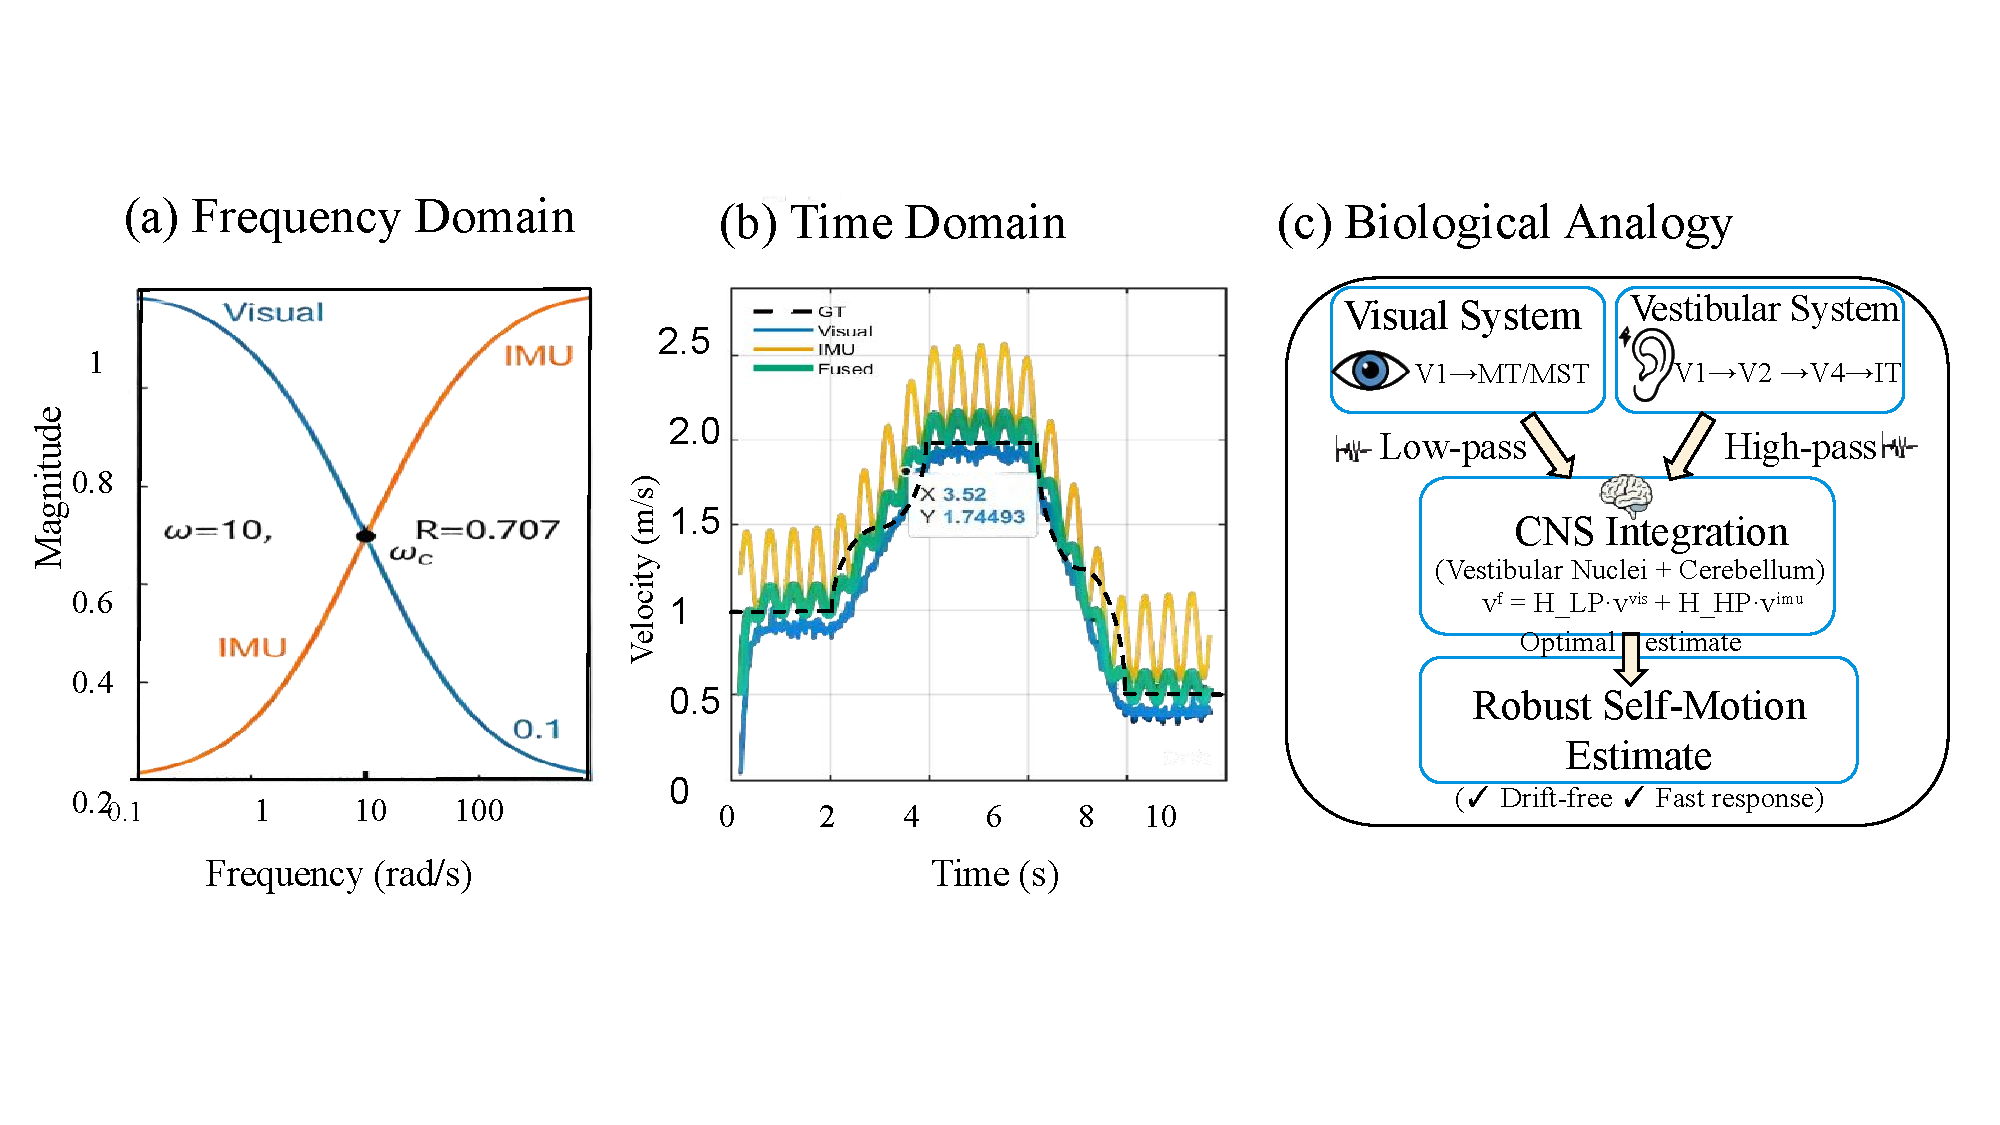
\includegraphics[width=\textwidth]{fig/imu_visual_complementary_fusion.pdf}
    \caption{互补IMU-视觉融合架构。(a) 展示互补滤波特性的频域分析。(b) 时域信号对比。(c) 中枢神经系统中前庭-视觉整合的生物学类比。}
    \label{fig:imu_visual_fusion}
\end{figure*}

\textbf{滤波器设计.} 设 $\mathcal{L}_\tau$ 表示时间常数为 $\tau$ 的低通滤波器，$\mathcal{H}_\tau$ 表示满足 $\mathcal{L}_\tau + \mathcal{H}_\tau = \mathrm{Id}$（单位算子）的互补高通滤波器。融合后的速度与偏航角速度为：
\begin{align}
    \text{低通: }  & \;L_t = \alpha L_{t-1} + (1-\alpha) x_t,\quad L_0=0 \\
    \text{高通: } & \;H_t = x_t - L_t
\end{align}
其中 $\alpha$ 为IIR滤波器遗忘因子，$L_t$ 存储低频平滑信号，$H_t$ 存储残余高频信号分量。

\textbf{生物学类比.} 该融合策略镜像了前庭核与后顶叶皮层（7a区）中的多感官整合，视觉与前庭信号在此结合以估计自运动。这些区域的神经元表现出视觉与前庭调制的加权组合，且权重随信号可靠性动态变化——类似于我们的固定权重参数 $\eta$ 与 $\eta_r$。

\textbf{离散时间实现.} 在采样间隔 $\Delta t$ 下，我们实现一阶IIR（无限脉冲响应）滤波器。选取遗忘因子 $\alpha=\exp(-\Delta t/\tau)$ 与 $\alpha_r=\exp(-\Delta t/\tau_r)$。对任意输入序列 $x_t$，定义：
\begin{align}
    \text{低通: }  & \;L_t = \alpha L_{t-1} + (1-\alpha) x_t,\quad L_0=0 \\
    \text{高通: } & \;H_t = x_t - L_t
\end{align}
则融合线索计算如下：
\begin{align}
    \mathbf{v}^\mathrm{f}_t & = (1-\eta)\,L^\mathrm{vis}_t + \eta\,H^\mathrm{imu}_t \\
    r^\mathrm{f}_t          & = (1-\eta_r)\,L^{r,vis}_t + \eta_r\,H^{r}_t
\end{align}
其中 $L^\mathrm{vis}_t$ 与 $H^\mathrm{imu}_t$ 分别表示低通滤波后的视觉速度与高通滤波后的IMU速度，偏航角速度同理。

\textbf{频域传递函数.} 在 $s = j\omega$（频率变量）的拉普拉斯域中，一阶低通与高通滤波器的传递函数为：
\begin{align}
    H_{LP}(s) & = \frac{1}{1 + \tau s} = \frac{1/\tau}{s + 1/\tau}, \label{eq:h_lp} \\
    H_{HP}(s) & = \frac{\tau s}{1 + \tau s} = \frac{s}{s + 1/\tau}, \label{eq:h_hp}
\end{align}
满足 $H_{LP}(s) + H_{HP}(s) = 1$（全频域单位增益）。截止频率 $\omega_c = 1/\tau$ 分隔低频与高频区域：当 $\omega \ll \omega_c$ 时，$|H_{LP}| \approx 1$ 且 $|H_{HP}| \approx 0$，视觉通路占主导（无漂移、动力学较慢）；而当 $\omega \gg \omega_c$ 时，$|H_{LP}| \approx 0$ 且 $|H_{HP}| \approx 1$，IMU线索占主导（快但漂移）。

取 $\tau = 0.1$ s 时，截止频率为 $\omega_c = 10$ rad/s（$\approx 1.6$ Hz），确保IMU处理高频运动（$>$2 Hz，如振动、快速转弯），而视觉校正低频漂移（$<$1 Hz）。这模仿了生物学前庭-视觉整合，其中前庭器官响应0.1-10 Hz的频率，而低于0.5 Hz时视觉运动感知占主导 \cite{Angelaki2004}。

\textbf{计算效率.} 该实现每个信号只需两个状态变量（当前低通滤波器状态 $L_t$ 与前值 $L_{t-1}$），仅涉及简单的标量乘法与加法。每次更新计算代价为 $\mathcal{O}(1)$，适合实时嵌入式实现——这与紧耦合视觉-惯性里程计的扩展卡尔曼滤波所需的 $\mathcal{O}(n^3)$ 矩阵求逆形成鲜明对比。

\textbf{自适应加权.} 虽然基线实现使用固定融合权重 $\eta$ 与 $\eta_r$，但该框架可自然扩展到基于信号可靠性的自适应加权。例如，在激烈机动或光照快速变化时，视觉里程计可能不可靠，应增加对IMU的依赖（$\eta \to 1$）。反之，在IMU积分累积偏置的慢速运动中，视觉里程计应占主导（$\eta \to 0$）。自适应方案可实现为：
\begin{equation}
    \eta_t = f(\sigma^\mathrm{vis}_t, \sigma^\mathrm{imu}_t),\quad \text{例如} \quad \eta_t = \frac{\sigma^\mathrm{vis}_t}{\sigma^\mathrm{vis}_t + \sigma^\mathrm{imu}_t}
\end{equation}
其中 $\sigma_t^\mathrm{vis}$ 与 $\sigma_t^\mathrm{imu}$ 为视觉与惯性测量的实时不确定性估计，$\eta_t$ 为时变融合权重。

此外，式~\eqref{eq:vis_scale} 中的视觉里程计尺度因子 $\kappa_t$ 可以自适应，以维持视觉与惯性速度幅值间的一致性：
\begin{equation}
    \kappa_{t+1} = \kappa_t \cdot \left(1 + \beta \frac{\lVert\mathbf{v}^\mathrm{imu}_t\rVert - \lVert\kappa_t \bar{\mathbf{v}}^\mathrm{vis}_t\rVert}{\lVert\kappa_t \bar{\mathbf{v}}^\mathrm{vis}_t\rVert}\right)
\end{equation}
其中 $\beta \ll 1$ 为在线视觉里程计尺度校正的小自适应增益（如 $\beta=0.01$）。该在线尺度自适应可补偿所设地面平面深度或相机标定不精确引起的系统误差。

\subsection{神经空间表征}

空间表征模块通过结合式位姿细胞（conjunctive pose cells）使用受生物启发的神经坐标系编码机器人的4自由度位姿。3D位置 $(x, y, z)$ 由使用3D连续吸引子网络（MD-CAN）的网格细胞表示，而朝向 $\psi$（偏航）由多层头方向细胞编码。这些表征通过吸引子动力学实现稳定、容噪的路径积分。

\textbf{3D网格细胞网络.} 3D网格细胞网络模仿哺乳动物大脑中的3D空间神经表征，表现出规则的3D晶格模式（面心立方，FCC），编码位置并为路径积分提供普适度量。受蝙蝠3D网格细胞发现~\cite{finkelstein2016three} 与六角形网格结构理论模型~\cite{hafting2005microstructure} 的启发，我们的实现在保持关键生物学性质（多尺度表征、度量路径积分、噪声鲁棒性）的同时，将2D连续吸引子网络扩展到完整3D空间。

\textbf{网络架构.} 3D网格细胞网络是维度为 $N_x \times N_y \times N_z$（典型取 $N_x = N_y = N_z = 61$）的3D多尺度连续吸引子网络（MD-CAN）。网络活动 $\mathbf{A}^\mathrm{g}_t \in \mathbb{R}^{N_x \times N_y \times N_z}$ 表示机器人3D位置 $(x_t, y_t, z_t)$ 的分布式群体编码，其中每个细胞 $(i,j,k)$ 调谐于环境中的某个偏好空间位置。活动形成以当前位置为中心局域化的“凸起”（或活动包），类似于啮齿动物内嗅皮层记录中观察到的活动凸起。

网络拓扑采用环面卷绕的周期性边界条件，实现无界空间表征。细胞间连接遵循面心立方（FCC）晶格——3D中最致密的球堆积——以最少神经元提供最优空间覆盖。在FCC结构中，每个细胞有12个最近邻（2D六角形网格中为6），从而得到各向同性方向敏感度的高效3D路径积分。

\begin{figure*}[!t]
    \centering
    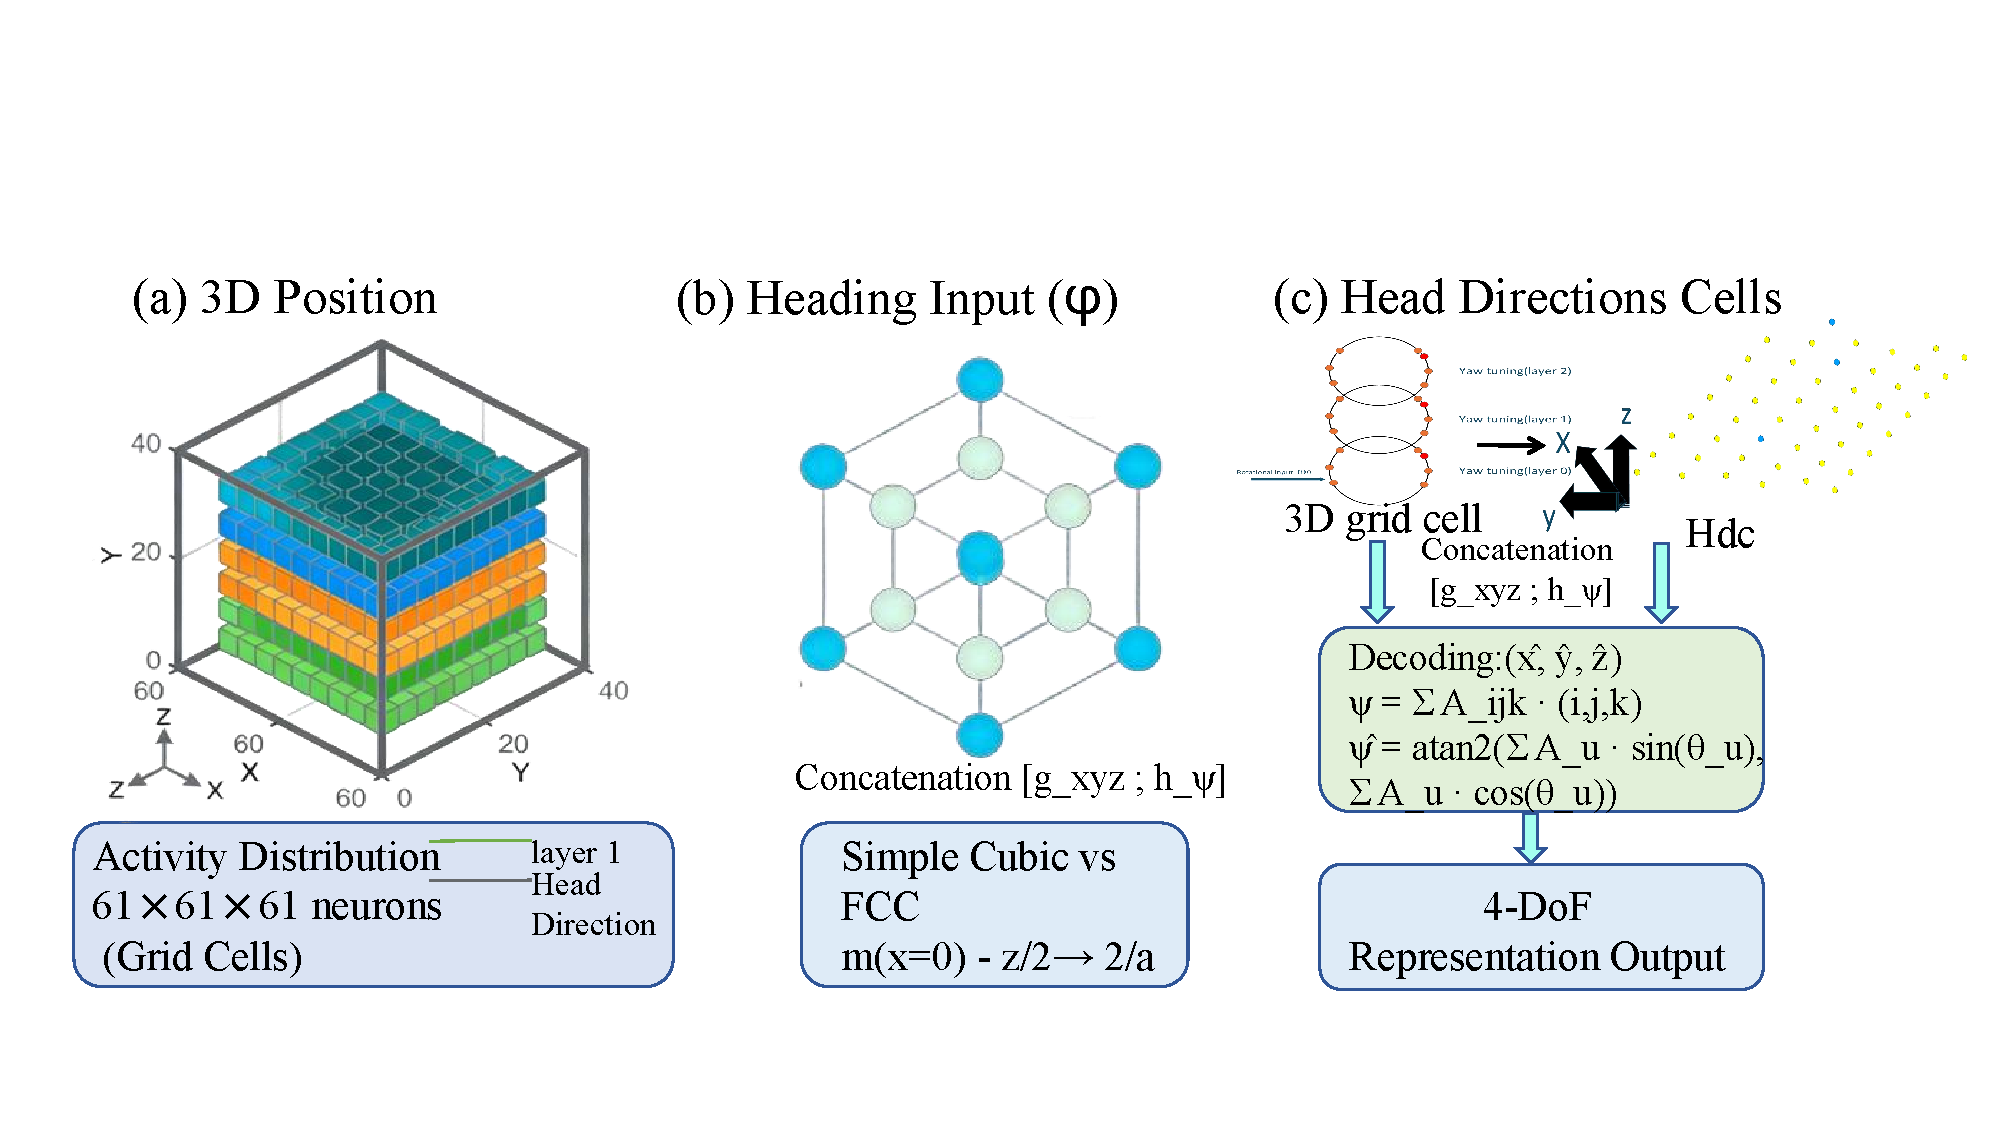
\includegraphics[width=\textwidth]{fig/3d_grid_cell_fcc_lattice.pdf}
    \caption{具有FCC晶格结构的3D网格细胞网络。(a) 通过分布式群体编码表示位置 $(x,y,z)$ 的3D活动包。(b) 展示三层高度实现的致密3D堆积、呈现六角形网格模式的FCC晶格结构。(c) 结合位置与朝向表征的4自由度编码方案。}
    \label{fig:3D_grid_cell_fcc}
\end{figure*}

图~\ref{fig:3D_grid_cell_fcc} 示意性地展示了：(a) 位置 $(x, y, z)$ 处的3D活动凸起，以等值面表示以可视化局域化兴奋；(b) FCC晶格投影到2D平面，展示由层间偏移排布产生的特征六角形模式，不同高度层（以颜色标示）平移半个晶格常数以实现最优堆积；(c) 集成位置与朝向表征的完整4自由度编码流水线。

\textbf{连续吸引子动力学.} 网络通过三个关键机制维持局域化的活动“凸起”：

\textbf{(1) 局域兴奋.} 细胞按高斯连接核兴奋其邻居。采用可分离核
\begin{equation}
    \mathcal{K}^\mathrm{g}_{a,b,c}=\mathcal{N}(a;0,\sigma_x)\mathcal{N}(b;0,\sigma_y)\mathcal{N}(c;0,\sigma_z)
\end{equation}
其中 $\mathcal{N}(\cdot;\mu,\sigma)$ 表示一维高斯分布，$\sigma_x,\sigma_y,\sigma_z$ 为三轴上的空间核宽度。
兴奋性更新为：
\begin{equation}
    \Delta A^\mathrm{g}_{i,j,k}=\sum_{p,q,r} A^\mathrm{g}_{p,q,r}\,\mathcal{K}^\mathrm{g}_{\langle i-p\rangle_{N_x},\langle j-q\rangle_{N_y},\langle k-r\rangle_{N_z}}
\end{equation}
其中 $\langle \cdot \rangle_N$ 表示周期性边界条件下的模 $N$ 卷绕。典型参数为 $\sigma_x = \sigma_y = \sigma_z = 5$ 个细胞。

\textbf{(2) 全局抑制与归一化.} 均匀全局抑制减去平均活动，整流与归一化维持单一稳定凸起：
\begin{equation}
    A^\mathrm{g}_{i,j,k}\leftarrow \big[A^\mathrm{g}_{i,j,k}+\Delta A^\mathrm{g}_{i,j,k}-\lambda\,\bar A^\mathrm{g}\big]_+,\quad \bar A^\mathrm{g}=\frac{1}{N_xN_yN_z}\sum_{p,q,r}A^\mathrm{g}_{p,q,r}
\end{equation}
其中 $[\cdot]_+ = \max(0, \cdot)$ 为整流，$\lambda$ 控制抑制强度（典型 $\lambda=1.0$）。抑制之后，活动做 $L_1$ 归一化：
\begin{equation}
    A^\mathrm{g}\leftarrow \frac{A^\mathrm{g}}{\lVert A^\mathrm{g}\rVert_1}=\frac{A^\mathrm{g}}{\sum_{i,j,k}|A^\mathrm{g}_{i,j,k}|}
\end{equation}
该归一化确保活动模式具有单位总质量，使读出（质心）对整体活动幅度不敏感。

\textbf{(3) 路径积分.} 活动凸起按融合速度线索 $\mathbf{v}^\mathrm{f}_t = (v^f_x, v^f_y, v^f_z)$ 移动。索引移动量计算为：
\begin{equation}
    (\Delta i,\Delta j,\Delta k)=\big(\lfloor \gamma_x v^f_x\Delta t\rfloor,\ \lfloor \gamma_y v^f_y\Delta t\rfloor,\ \lfloor \gamma_z v^f_z\Delta t\rfloor\big)
\end{equation}
其中 $\gamma_x,\gamma_y,\gamma_z$ 为度量-索引增益因子，将物理速度转换为网络网格移动。
\begin{equation}
    A^\mathrm{g}_{i,j,k}\leftarrow A^\mathrm{g}_{\langle i-\Delta i\rangle_{N_x},\langle j-\Delta j\rangle_{N_y},\langle k-\Delta k\rangle_{N_z}}
\end{equation}
该离散移动操作在环面网络拓扑上高效实现了路径积分。

\textbf{视觉锚定与漂移校正.} 纯路径积分会随时间累积漂移。为防止误差无界增长，网格细胞活动通过学习到的关联锚定到视觉地标。设 $\Xi_{m,i,j,k}$ 存储视觉模板 $m$ 与网格细胞 $(i,j,k)$ 之间的关联强度。对每个激活的视觉模板 $m \in \mathcal{S}_{active}$，更新关联并注入校正活动：
\begin{align}
     & \text{Hebbian学习: } \Xi_{m,i,j,k}^{t+1}=\max\big(\eta\,VT_m\,A^\mathrm{g}_{i,j,k},\ \Xi_{m,i,j,k}^{t}\big)                                             \\
     & \text{校正注入: } \Delta A^\mathrm{g}_{i,j,k} \mathrel{+}= \frac{\rho}{|\mathcal{S}_{active}|}\sum_{m\in\mathcal{S}_{active}}VT_m\,\Xi_{m,i,j,k}
\end{align}
其中 $\eta$ 为Hebbian学习率，$\rho$ 为空间校正强度，$\mathcal{S}_{active}$ 为当前匹配的视觉模板集合。

\textbf{多层头方向细胞.} 多层头方向细胞（HDC）网络使用维度为 $N_\psi \times N_h$（方位角分箱 $\times$ 高度层）的2D MD-CAN表示机器人的朝向。不同高度层允许表示不同垂直位置处的朝向，支持朝向可能随高度变化的3D运行。

\textbf{网络架构.} 多层头方向网络的活动为 $\mathbf{A}^\mathrm{h} \in \mathbb{R}^{N_\psi \times N_h}$（典型取 $N_\psi = 360$ 个方位角分箱，$N_h = 5$ 个高度层）。每个细胞 $(u, h)$ 调谐于方位角 $\theta_u = 2\pi u / N_\psi$ 与高度层 $h$。

\textbf{吸引子动力学.} 与网格细胞网络类似，HDC网络采用局域兴奋、全局抑制与路径积分。采用高斯核 $\mathcal{K}^\mathrm{h}$：
\begin{equation}
    \Delta A^\mathrm{h}_{\psi,h}=\sum_{u,v}A^\mathrm{h}_{u,v}\,\mathcal{K}^\mathrm{h}_{\langle \psi-u\rangle_{N_\psi},\langle h-v\rangle_{N_h}}
\end{equation}
随后进行抑制与归一化：
\begin{equation}
    A^\mathrm{h}\leftarrow \frac{[A^\mathrm{h}+\Delta A^\mathrm{h}-\lambda_h\,\bar A^\mathrm{h}]_+}{\lVert A^\mathrm{h}\rVert_1}
\end{equation}
路径积分按偏航角速度 $r^f$ 与垂向速度 $v^f_z$ 移动活动凸起：
\begin{equation}
    \Delta\psi=\lfloor \gamma_\psi r^f \Delta t\rfloor,\quad \Delta h=\lfloor \gamma_h v^f_z \Delta t\rfloor
\end{equation}
其中 $\gamma_\psi$ 将角速度转换为方位角分箱，$\gamma_h$ 将垂向速度映射为高度层移动量。

\textbf{位姿读出.} 度量位姿估计通过质心计算（群体向量解码）从空间细胞活动中解码得到：
\begin{align}
    \hat{\mathbf{p}}_t & = ({\hat x}_t, {\hat y}_t, {\hat z}_t) = \frac{\sum_{i,j,k} \mathbf{c}_{i,j,k} A^\mathrm{g}_{i,j,k,t}}{\sum_{i,j,k} A^\mathrm{g}_{i,j,k,t}}, \quad \mathbf{c}_{i,j,k} = (x_i, y_j, z_k) \\
    \hat{\psi}_t       & = \mathrm{atan2}\left(\sum_{u,h} A^\mathrm{h}_{u,h,t} \sin\theta_u, \sum_{u,h} A^\mathrm{h}_{u,h,t} \cos\theta_u\right), \quad \theta_u = 2\pi u / N_\psi
\end{align}
该解码天然处理朝向的环形拓扑（使用 $\mathrm{atan2}$ 避免角度回绕问题），并通过加权平均为位置提供亚分箱分辨率。

\subsection{经验地图与闭环}

多层经验地图将3D空间经验表示为图结构，提供一种混合拓扑-度量表征，兼具离散基于地点的地图（拓扑鲁棒性、闭环）与连续度量表征（精确定位）的优点。

\textbf{经验表征.} 每个经验节点 $\mathcal{E}_i$ 编码一段独立的空间情节，包含激活的视觉模板与描述子 $(VT_i,\,\boldsymbol{\phi}_i\in\mathbb{R}^{4096})$、同步的空间细胞编码 $\mathbf{P}^{gc}_i=\mathbf{A}^\mathrm{g}_i\in\mathbb{R}^{N_x\times N_y\times N_z}$ 与 $\mathbf{P}^{hdc}_i=\mathbf{A}^\mathrm{h}_i\in\mathbb{R}^{N_\psi\times N_h}$、从这些活动解码出的度量位姿 $(x_i, y_i, z_i, \psi_i)$，以及用于时序排序的时间戳 $t_i$。
这种丰富的多模态编码通过视觉匹配实现鲁棒的闭环检测，同时通过空间细胞编码保持度量信息。

\textbf{经验创建与连接.} 随着机器人导航，当当前空间表征与所有现有经验都足够不同时，创建新经验。创建准则综合视觉与空间细胞相似度：
\begin{equation}
    \begin{aligned}
        \text{若 }\; & d_{cos}(\boldsymbol{\phi}_t, \boldsymbol{\phi}_j) > \tau_{VT} \quad \text{对所有 } j \in \mathcal{E} \\
                                           & \text{或 } \lVert (\hat{x}_t, \hat{y}_t, \hat{z}_t) - (x_j, y_j, z_j) \rVert > d_{thresh} \text{ 则创建新经验}
    \end{aligned}
\end{equation}
其中 $\tau_{VT} = 0.08$ 为视觉模板匹配阈值，$d_{thresh}$ 为空间距离阈值（典型 0.5~m）。

相邻经验由编码相对位姿转移的有向边连接：
\begin{equation}
    \mathbf{T}_{i \to i+1} = (\Delta x, \Delta y, \Delta z, \Delta \psi) = (x_{i+1} - x_i, y_{i+1} - y_i, z_{i+1} - z_i, \psi_{i+1} - \psi_i)
\end{equation}
这些边构成经验地图图 $\mathcal{G} = (\mathcal{V}, \mathcal{E})$ 的主要拓扑结构。

\textbf{闭环检测.} 当当前视觉模板与某历史经验匹配超过最小时间间隔（以避免平凡闭环）时，检测到闭环：
\begin{equation}
    \begin{aligned}
        \text{若存在 } j:\; & d_{cos}(\boldsymbol{\phi}_t, \boldsymbol{\phi}_j) < \tau_{loop} \\
                                                      & |t - t_j| > T_{min} \text{ 则检测到闭环}
    \end{aligned}
\end{equation}
其中 $\tau_{loop} = 0.05$（比模板创建阈值更严格，以减少误报），$T_{min} = 50$ 帧（10 Hz下约5秒）。

检测到闭环后，向图中添加一条带位姿残差的闭环边：
\begin{equation}
    \mathbf{T}_{loop} = (\hat{x}_t - x_j, \hat{y}_t - y_j, \hat{z}_t - z_j, \hat{\psi}_t - \psi_j)
\end{equation}
该闭环约束通常违背图一致性（由于累积漂移），从而触发地图松弛。

\textbf{地图松弛.} 地图松弛将闭环误差分布到闭环路径上的所有经验，以最小化全局不一致。我们采用迭代松弛算法：

\textbf{第1步：识别闭环路径.} 给定从经验 $j$ 到经验 $t$ 的闭环边，识别沿路径的经验序列 $\mathcal{P} = \{j, j+1, \ldots, t-1, t\}$。

\textbf{第2步：计算位姿残差.} 沿闭环累积的位姿转移理想情况下应当闭合（回到原点）：
\begin{equation}
    \mathbf{e}_{loop} = \sum_{k \in \mathcal{P}} \mathbf{T}_{k \to k+1} - \mathbf{T}_{loop}
\end{equation}
其中 $\mathbf{e}_{loop}$ 为闭合轨迹周围的累积位姿漂移残差，$\mathcal{P}$ 表示构成闭环的有序经验序列。

\textbf{第3步：分布校正.} 将校正量按比例分布到闭环经验上：
\begin{equation}
    \mathbf{T}_{k \to k+1} \leftarrow \mathbf{T}_{k \to k+1} - \frac{\mathbf{e}_{loop}}{|\mathcal{P}|}
\end{equation}
该均匀分布假设漂移以恒定速率累积，是一个合理的一阶近似。

\textbf{第4步：更新经验位姿.} 通过对校正后的转移量积分，重新计算所有经验位姿：
\begin{equation}
    (x_{k+1}, y_{k+1}, z_{k+1}, \psi_{k+1}) = (x_k, y_k, z_k, \psi_k) + \mathbf{T}_{k \to k+1}
\end{equation}

\textbf{第5步：重新锚定空间细胞.} 将校正后的位姿 $(\hat{x}, \hat{y}, \hat{z}, \hat{\psi})_{corr}$ 通过在校正位置处重新初始化活动凸起，重新注入空间细胞网络。这从校正后的参考点“重置”路径积分，防止后续运行中误差累积。

该松弛过程迭代运行直至收敛或达到最大迭代次数，确保经验地图保持全局一致，同时保留局部度量精度。
